\begin{frame}[c,parent={cmap:jabuti-software-testing},hasnext=true,hasprev=false]
\label{cmap:jabuti-slicing-tool}
\label{cmap:slicing-tool}
\frametitle{Slicing tool}

\insertcmap{Courses-SoftwareTesting-JaBUTi-JaBUTiToolsProgramSlicing}
\end{frame}


\begin{frame}[parent={cmap:jabuti-slicing-tool},hasnext=true,hasprev=true]
\label{concept:program-slicing}
\label{concept:software-slicing}
\frametitle{Slicing tool}

\begin{block:concept}{Slicing tool}
\begin{itemize}
	\item Slicing tool uses program slicing to highlight, for a given set of
	successful and failure test cases, the parts of the program under testing
	that have a higher probability of having a fault.
\end{itemize}
\end{block:concept}

\begin{block:concept}{Program slicing}
\begin{itemize}
	\item Program slicing can be used to help engineers to understand code.
	\begin{itemize}
		\item A backward slice from a point in the program identifies all parts
		of the code that contribute to that point.

		\item A forward slice identifies all parts of the code that can be
		affected by the modification to the code at the slice point.
	\end{itemize}
\end{itemize}
\end{block:concept}
\end{frame}


\begin{frame}
\frametitle{Program slicing}

\begin{block:ie}{Example}
\begin{itemize}
	\item Suppose a proposed program modification only changes the value of
	variable $v$ at program point $p$.

	\item If the forward slice with respect to $v$ and $p$ is disjoint from the
	coverage of a test set $t$, then test set $t$ does not have to be rerun.

	\item Suppose a coverage tool reveals that a use of variable $v$ at program
	point $p$ has not been tested.

	\item The input date required to cover $p$ can be found in the backward
	slice of $v$ with respect to $p$.
\end{itemize}
\end{block:ie}
\end{frame}



\begin{frame}
\frametitle{Slicing tool}

\begin{block}{Static and dynamic slice}
\begin{itemize}
	\item An important distinction exists between a static and a dynamic slice.

	\item Static slices are computed without making assumptions regarding a
	program's input, which provides the set of all statements that might affect
	the value of a given variable.

	\item Dynamic slices relies on a the execution trace information of the
	software, providing all statements that actually affect the value of
	a variable.
\end{itemize}
\end{block}

\begin{block}{}
\begin{itemize}
	\item Using dynamic tracing, JaBUTi can be used to find the fault
	triggered by a failed test case.
\end{itemize}
\end{block}
\end{frame}




\begin{frame}[parent={cmap:jabuti-slicing-tool},hasnext=true,hasprev=true]
\frametitle{Slicing tool}
\label{concept:slicing-tool}
\label{concept:jabuti-slicing-tool}
\label{concept:software-slicing-tool}

\begin{block:fact}{Slicing tool}
\begin{itemize}
	\item Slicing tool is available through the \srccode{Tools/Slicing Tool}
	menu option.

	\item By changing to the slicing tool, the tester has to choose, among
	the test cases:
	\begin{itemize}
		\item the ones that cause the fault;
		\item and the ones that do not reveal the fault.
	\end{itemize}

	\item Based on the execution path of the failed and successful test cases,
	the tool highlights the part of the code that have a higher probability of
	containing the fault.
\end{itemize}
\end{block:fact}
\end{frame}


\begin{frame}
\frametitle{Slicing tool}

\begin{block:fact}{Slicing tool}
\begin{itemize}
	\item JaBUTi uses a simple dynamic slice criterion, based on
	control-flow information, to identify a subset of statements that
	probably contain the fault.

	\item The idea is to compute:
	\begin{itemize}
		\item the failed set $F_S$ of BG nodes (the execution path) of a
		failed test case (which includes all statements executed by the failed
		test case)

		\item the successful set $S_S$ of BG nodes considering successful test
		cases,

		\item the difference and the intersection of these sets to establish to
		prioritize the statements executed by the failed test case that are
		candidate to trigger the failure.
	\end{itemize}
\end{itemize}
\end{block:fact}
\end{frame}



\begin{frame}
\frametitle{Slicing tool}

\begin{block:fact}{Slicing tool}
\begin{itemize}
	\item Using such approach, instead of the complete set of BG nodes $N$
	(which represents all statements of a method), the tester has only to
	consider the subset of BG nodes present in $F_S$
	\begin{itemize}
		\item The other BG nodes contains the statements not executed by the
		failed test case and that cannot contain the fault.
	\end{itemize}

	\item Moreover, considering the subset of nodes executed by the successful
	test cases, the most probably location of the fault is in the
	statements executed by the failed test case but not executed by
	the successful test cases, \textit{i.e.}, the subset $F_S \setminus S_S$.
\end{itemize}
\end{block:fact}
\end{frame}



\begin{frame}
\frametitle{Slicing tool}

\begin{block}{Example}
Consider the BG presented below. It represents a program that outputs the
average of the numbers in an array.
\end{block}

\begin{block}{Average}
\centering
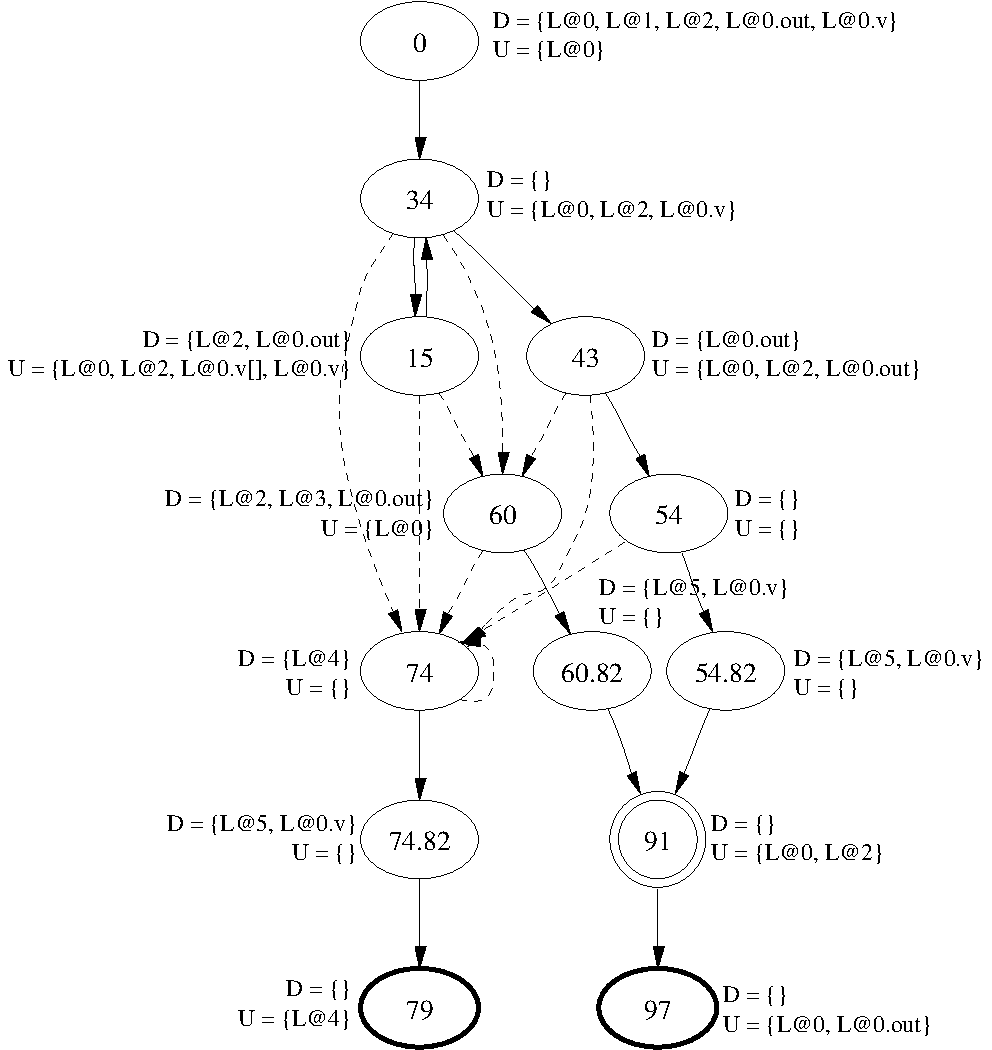
\includegraphics[width=4.5cm]{resources/aux/examples/average/average-bcfg.pdf}
\end{block}
\end{frame}


\begin{frame}
\frametitle{Slicing tool}

\begin{block}{Example}
\begin{enumerate}
	\item $N$ is the complete set of BG nodes ($N = \{0, 15, 34, 43, 54,
	54.82, 60, 60.82, 74, 74.82, 79, 91, 97\}$).

	\item Suppose a failed test case that goes though BG nodes
	$F_S = \{0, 34, 15, 34, 43, 54, 54.82, 91, 97\}$ and a successful
	test case that goes through BG nodes $S_S = \{0, 34, 43, 60,
	60.82, 91, 97\}$.

	\item The most probably locations for the fault are in
	the statements in nodes 15, 54 or 54.82, since they are only
	executed by the faulty test case ($F_S \setminus S_S$).

	\item If the fault is not located on such statements, it will be found in
	the other statements that compose the BG nodes 0, 34, 43, 91 and 97
	($F_S \cap S_S$). All the other BG nodes have not to be analyzed.
\end{enumerate}
\end{block}
\end{frame}



\begin{frame}[hasnext=false]
\frametitle{Slicing tool}

\begin{block}{Example}
\insertmovie{resources/JaBUTi/JaBUTi-VendingMachine/JaBUTi-VendingMachine-SlicingTool/JaBUTi-VendingMachine-SlicingTool}
\end{block}
\end{frame}
